\PassOptionsToPackage{unicode}{hyperref}
\documentclass[aspectratio=1610, 9pt]{beamer}

% Load packages you need here
\usepackage{polyglossia}
\setmainlanguage{german}

\usepackage{csquotes}
\usepackage{graphicx}
\usepackage{siunitx}
\usepackage{amsmath}
\usepackage{amssymb}
\usepackage{mathtools}

\usepackage{hyperref}
\usepackage{bookmark}

% load the theme after all packages

\usetheme[
  showtotalframes, % show total number of frames in the footline
  % dark, % optional dark theme, uncomment to use
]{tudo}

% Put settings here, like
\unimathsetup{
  math-style=ISO,
  bold-style=ISO,
  nabla=upright,
  partial=upright,
  mathrm=sym,
}
\begin{document}
\begin{frame}
    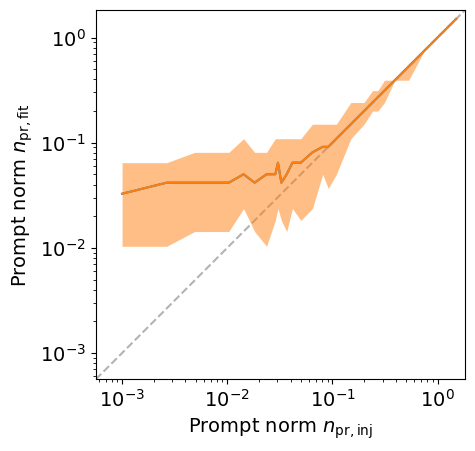
\includegraphics[width=0.6\textwidth]{../Plots/bias}
\end{frame}
\begin{frame}
    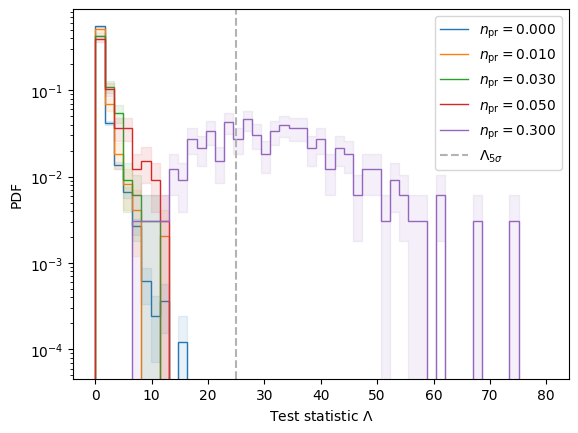
\includegraphics[width=0.7\textwidth]{../Plots/test_statistic}
\end{frame}
\begin{frame}
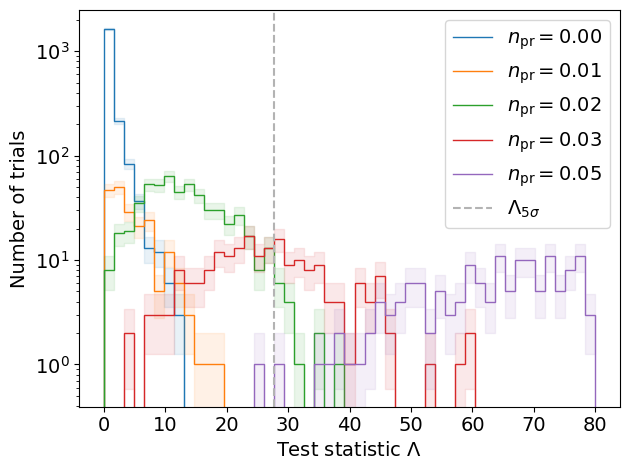
\includegraphics[width=0.7\textwidth]{../Plots/test_statisti_previous}
\end{frame}
\end{document}